\begin{frame}
\frametitle{Эксперимент: Causal World, описание среды}

\begin{columns}[t]
\begin{column}{0.33\linewidth}<3->
    Сырое изображение из среды::
    % \begin{itemize}
    %     \item Each observation contains two entities of interest
    %     \item Each entity have its own dynamics
    %     \item Actor can directly affect or have a long-term influence over object
    % \end{itemize}
            \begin{figure}
            \begin{subfigure}{0.8\linewidth}
                \centering
                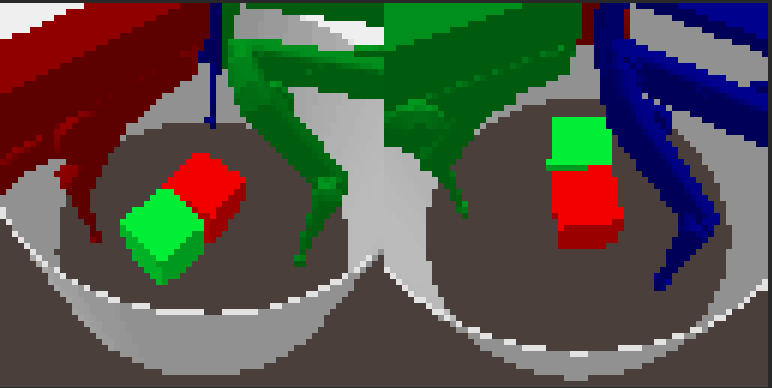
\includegraphics[width=\linewidth]{images/env/causal_world/actual_obs.png}
            \end{subfigure}
            \end{figure}
\end{column}
\hfill
\begin{column}{0.63\linewidth}<1->
    Пример наблюдений:
    \begin{figure}
    \onslide<1->{\begin{subfigure}{.4\linewidth}
        \centering
            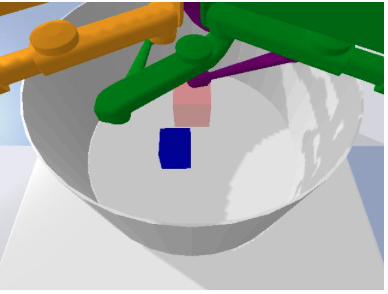
\includegraphics[width=\linewidth]{images/env/causal_world/obs_1.png}
    \end{subfigure}}
    \end{figure}
    \begin{figure}
        \onslide<1->{\begin{subfigure}{.4\linewidth}
            \centering
                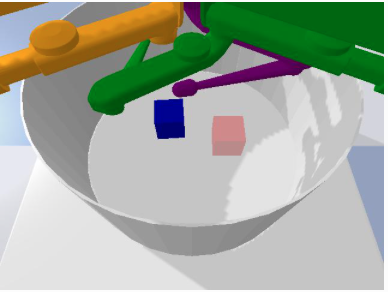
\includegraphics[width=\linewidth]{images/env/causal_world/obs_2.png}
        \end{subfigure}}
        \hspace{3em}%
        \onslide<1->{\begin{subfigure}{.4\linewidth}
            \centering
                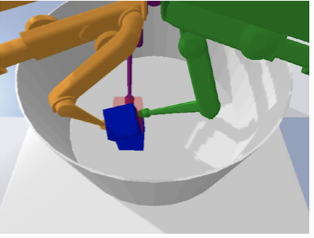
\includegraphics[width=\linewidth]{images/env/causal_world/obs_3.png}
        \end{subfigure}}
    \end{figure}
    
    % Probably not needed
    % \begin{itemize}
    %     \item The task is defined by drawer position
    %     \item Ground truth segmentation masks
    %     \item Out-of-distribution test tasks
    %     \item Single topdown camera for all tasks
    % \end{itemize}
\end{column}
\end{columns}
\note[item]<1->{We built the custom parameterized task environment for evaluating the generalization capabilities of algorithm. It is a drawer, which should be opened by robotic hand.In each specific task, the drawer is fixed.}
\end{frame}